\documentclass[12pt,twoside, a4paper, twocolumn]{article}
\usepackage[utf8]{inputenc}
\usepackage[brazil]{babel}
\usepackage[margin = 0.5in]{geometry}
\usepackage{amsmath}
\usepackage{amsthm}
\usepackage{amssymb}
\usepackage{amsthm}
\usepackage{setspace}
\usepackage[americanvoltages,fulldiodes,siunitx]{circuitikz}
\usepackage{lipsum}
\usepackage{pgfplots}
\usepackage{ifthen}
\usepackage{adjustbox}
\usepackage[section]{placeins}
\usepackage{hyperref}
\usepackage{graphicx}
\pgfplotsset{compat=newest}
\graphicspath{ {./images/} }


%  #1 color - optional #2 x_0 #3 y_0 #4 x_f #5 y_f #6 name - optional  #7 true if adding lines to axis

\newcommand{\drawvector} [9] [color=cyan] {
    \draw[line width=1.5pt,#1,-stealth](axis cs: #2, #3)--(axis cs: #4, #5) node[anchor=south west]{$#6$};

    

\ifthenelse{\equal{#7}{true}}{
    \draw[line width=1pt,#1, dashed](axis cs: #4, #5)--(axis cs: #4, 0) node[anchor= north west]{$#8$};
    \draw[line width=1pt,#1, dashed](axis cs: #4, #5)--(axis cs: 0, #5) node[anchor=south east]{$#9$};
    }
    {}
}

\newcommand\deriv[2]{\frac{\mathrm d #1}{\mathrm d #2}}


\title{Primeiro Relatório de Lab de Circuitos}
\author{Henrique da Silva \\ hpsilva@proton.me}
\date{\today}
\pgfplotsset{width = 10cm, compat = 1.9}


\begin{document}
\maketitle
\pagenumbering{gobble}
\newpage
%pagenumbering{roman}
\tableofcontents
\newpage

\section{Introdução}

\paragraph*{Neste relatório, vamos discutir a ponte de Wheatstone e um método experimental para obter uma resistência desconhecida a partir de um circuito ja conhecido }

\paragraph*{Todos arquivos utilizados para criar este relatório, e o relatório em si estão em:  \url{https://github.com/Shapis/ufpe_ee/tree/main/4th semester/fisica experimental 2}}

\subsection{A ponte de Wheatstone}
\subparagraph*{}
\begin{center}
    \begin{circuitikz}
        \draw
        (-1,4) to[battery1=$V_{cc}$] (5,4) % l=5<\milli\volt>
        -- (5,0) -- (3.5,0) to [R, a=$R_2$] (2,2) to [R, a=$R_1$] (0.5,0) -- (-1,0) -- (-1,4)
        ;
        \draw (3.5,0) to [R=$R_x$] (2,-2) to [R, l=$R_k$] (0.5,0);
        \draw (2,2) to[rmeter, t=A] (2,-2);
        \draw (5,-0.05)
        node[rground]{};
        \draw (2,2)
        node[ocirc,  label=3:$A$]{};
        \draw (2,-2)
        node[ocirc,  label=-50:$B$]{};
        \draw (3.5,0)
        node[ocirc,  label=50:$D$]{};
        \draw (0.5,0)
        node[ocirc,  label=120:$C$]{};

    \end{circuitikz}
\end{center}

\subparagraph*{Esta tem como função principal determinar uma resistência desconhecida $R_x$ a partir de três resistências e uma corrente previamente conhecidas, que vamos chamar aqui de $A$ e $R_1$, $R_2$, e $R_k$.}

\subsection{Obtendo $R_x$}

\subparagraph*{Para obter essa resistência desconhecida, o que faremos é inicialmente determinar a corrente $A$. E tentar modificar a resistencia $R_k$ ate esta corrente $A$ se aproximar de $0$}

\subparagraph*{A ideia central disto eh que a corrente que esta saindo da fonte vai se dividir em $C$, e se $R_1 * R_x = R_k * R_2$ entao o sistema estara balanceado e a corrente $A$ sera 0.}

\subparagraph*{Ja que escolhemos o valor de $R_1$, $R_2$, e $R_k$, vamos poder determinar $R_x$ como a seguinte equacao:}


\begin{equation}
    \begin{aligned}
         & R_1 * R_x  = R_k * R_2       \\
         & R_x = \frac{R_2 * R_k}{R_1 } \\
    \end{aligned}
\end{equation}

\subparagraph*{Apesar de termos escolhido $R_1$ e $R_2$ iguais, nao simplifiquei a equacao para $R_x = R_k$. Porque perderia as incertezas de $R_1$ e $R_2$. }




\section{Tarefas}

\subsection{Aument a tensao da fonte ate a corrente em A atingir 9mA}

\subparagraph*{Fizemos isto com um $R_k$ fixo em $0$. E conseguimos uma tensao de $0.9V \pm 0.1V$ nos terminais da fonte}

\subsection{Varie a resistencia $R_k$ ate balancear a ponte de Wheatstone}

\subparagraph*{Neste caso a resistencia $R_x$ se iguala a resistencia $R_k$, obedecendo as devidas regras de derivacao de erro a partir dos erros conhecidos conseguimos:}

\begin{equation}
    R_k = (5.6 \pm 0.1) * 10^3 \varOmega
\end{equation}

\subsection{Com a ponte balanceada, aumente a tensao da fonte}

\paragraph*{Ela se manteve em zero.}

\paragraph*{O amperimetro vai estar medindo uma porcentagem de desbalanceamento na ponte. }

\paragraph*{Se a corrente que entra em $C$ aumenta, e a ponte esta desbalanceada. A corrente passando pelo amperimetro tambem aumenta.}

\paragraph*{No nosso caso em particular, nao foi possivel detectar este aumento, porem se constinuassemos aumentando a tensao da fonte, eventualmente veriamos o residuo do desbalanceamento passando pelo amperimetro.}

\subsection{Verifique o funcionamento com um resistor de $12k \varOmega$}

\paragraph*{Fizemos a verificacao, e conseguimos igualar o $R_k$ a $12k \varOmega$ resultando em uma corrente minima passando por $A$. }

\paragraph*{Esta corrente minima estava na ordem de $10^-6 A$, ela existe por causa dos erros associados as medidas do circuito. Em um circuito ideal ela seria 0.}

\subsection{Medindo resistencia da lampada}

\subsubsection{Tabela de dados}

\begin{center}
    \begin{tabular}{ |cc| }
        \hline
        Tensão (V)       & Resistencia L ($\varOmega$) \\
        $2.00$ $\pm0.05$ & $9$ $\pm1$                  \\
        $4.00$ $\pm0.05$ & $13$ $\pm1$                 \\
        $6.00$ $\pm0.05$ & $15$ $\pm1$                 \\
        \hline
    \end{tabular}
\end{center}

\subsubsection{Grafico}

\begin{adjustbox}{scale=0.70}
    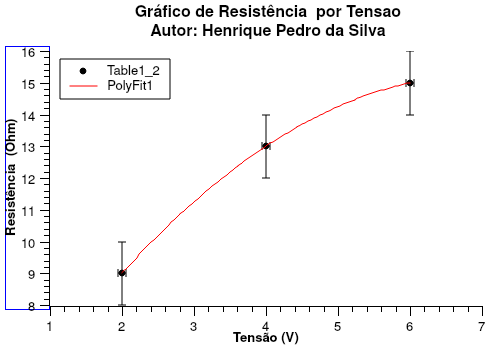
\includegraphics{Graph2.png}
\end{adjustbox}

\subsubsection{Interpretacao de resultados}

\subparagraph*{O resultado eh coerente com o esperado. Que seria o caso da lampada ser um caso de comportamento nao Ohmico, e que sua resistencia sobe de acordo com a tensao aplicada.}


\subsection{Comportamento do LDR}

\subparagraph*{Aplicamos uma tensao de $1.00V \pm 0.05$ no circuito, que resultou em uma corrente de $10.06mA \pm 0.1mA$ entrando no LDR antes do balanceamento.}

\subsubsection{Balanceamento com luz aplicada}

\subparagraph*{Neste caso conseguimos uma resistencia de $1.7*10^{3} \varOmega \pm 10^2 \varOmega$}

\subsubsection{Balanceamento sem luz aplicada}

\subparagraph*{Neste caso conseguimos uma resistencia de $7*10^{4} \varOmega \pm 10^4 \varOmega$}

\subsubsection{Interpretacao de resultados}

\subparagraph*{Podemos observar que a resistencia aumenta uma ordem de magnitude quando a luz eh removida. }

\subparagraph{Tambem foi observado que o sistema eh extremamente sensivel a mudancas pequenas de luz. Uma "sombra" leve ja faz a resistencia variar significantemente.}

\section{Conclusão}

\subparagraph*{Utilizando um circuito de \emph{Wheatstone} posso medir pequenas alterações de $corrente$ para descobrir uma resistência desconhecida com bastante precisão.}

\subparagraph*{Esse sistema é bastante robusto para diferentes valores de tensões de fonte. E tambem é significantemente resistente a erros aleatórios de medição.}
\end{document}

